\chapter{Processi Markoviani}
\section{Processi stocastici}
Introdurremo dei modelli probabilistici che permettono di descrivere un mondo
che cambia nel corso del tempo. Per fare ciò, avremo bisogno di una serie di
variabili casuali descritte da uno stato che varia nel tempo. Le relazioni tra i
cambiamenti di stato nel tempo descrivono l'evoluzione della variabile.

Possiamo quindi distinguere due tipologie di modelli:
\begin{itemize}
    \item \textbf{Statici}: il valore delle variabili non cambia nel tempo.
    \item \textbf{Dinamici}: il valore delle variabili cambia nel tempo. In questa
          tipologia, lo stato corrente dipende dalla storia e il processo di
          cambiamento è descritto da una serie di fotografie, o anche dette
          \textit{time slice}, ognuna delle quali contiene un insieme di variabili
          casuali.
\end{itemize}
\begin{definizione}[\textbf{Processo stocastico}]
    Un \textbf{processo stocastico} $\{X(t), t\in T\}$ è un insieme di variabili
    aleatorie che evolve nel tempo. Nello specifico, $X(t)$ rappresenta il valore
    della variabile aleatoria al tempo $t$.
\end{definizione}
Il tempo espresso dagli indici $t$ possono essere continui o discreti, inoltre
possono essere finiti o infiniti.

Avremo quindi diverse tipologie di processi stocastici:
\begin{itemize}
    \item Processi stocastici a tempo continuo:
          \begin{equation*}
              \{X(t), t>0\}
          \end{equation*}
    \item Processi stocastici a tempo discreto:
          \begin{equation*}
              \{X(t), t=0,1,\dots\}
          \end{equation*}
    \item Processi stocastici a stati continui:
          \begin{equation*}
              \{X(t), t=0,1,\dots\}, X(t) \text{ distribuzione continua}
          \end{equation*}
    \item Processi stocastici a stati discreti:
          \begin{equation*}
              \{X(t), t=0,1,\dots\}, X(t) \text{ distribuzione discreta}
          \end{equation*}
\end{itemize}
La variabile $X(t)$ è un valore dato dal sistema al tempo $t$, cioè un valore
della variabile che descrive uno stato del sistema al tempo $t$. Questo stato
può essere puntuale o cumulativo.
\begin{esempio}
    $X(t)$ può rappresentare il numero di visitatori fino al tempo $t$ (cumulativo),
    oppure può rappresentare il numero di visitatori al tempo $t$ (puntuale).
\end{esempio}
Un esempio di processo stocastico naive è il \textbf{Random Walk}, questo processo
viene descritto dalla seguente equazione:
\begin{equation*}
    X(t) = X(t-1) + \varepsilon_t
\end{equation*}
dove $\varepsilon_t \in \{-1, 1\}$,  $P(\varepsilon_t = -1) = p$ e $P(\varepsilon_t = 1) = 1- p$.
Se $p=\frac{1}{2}$ allora il processo è bilanciato, altrimenti il modello verrebbe
chiamato random walk con \textbf{drift}.

Un modo per generalizzare questo processo è quello di esprimere la distribuzione
$\varepsilon_t$ come continua, ad esempio $\varepsilon_t \approx N(0, 1)$. Questo
crea una randomicità maggiore.

Un'altro esempio di processo stocastico è il \textbf{processo autoregressivo del
    primo ordine} (\textit{first order autoregressive process}), il quale è descritto
dalla seguente equazione:
\begin{equation*}
    X_t = \alpha X_{t-1} + b + \varepsilon_t
\end{equation*}
con $\alpha,b$ constanti, con $-1<\alpha<1$ e $\varepsilon_t \approx N(0,1)$.

I processi stocastici sono importanti perché posso effettuare delle predizioni.
Per esempio il tracking degli oggetti in movimento nei video, oltre al tracking
possono essere utilizzati anche per generare dei processi (ex: generazioni di
comportamenti casuali per le simulazioni).
\section{Catene di Markov}
I processi stocastici possono rispettare una proprietà chiamata \textbf{proprietà
    Markoviana del primo ordine}, la proprietà assicura che la distribuzione di
probabilità per tutti i possibili valori futuri del processo dipende solo dal
valore corrente e non dai valori passati o da altre informazioni.

La generalizzazione di questa proprietà specifica il fatto che la distribuzione
di probabilità per tutti i possibili valori futuri del processo dipende da una
storia finita.

Tale proprietà può essere espressa in formule come:
\begin{equation}
    P(X_{t+1} = i_{t+1 } | X_t =i_t, \dots, X_{0} = i_{0})=P(X_{t+1} = i_{t+1 } | X_t =i_t)
\end{equation}
I processi stocastici che rispettano la \textbf{proprietà Markoviana} sono detti
\textbf{processi Markoviani} e verranno rappresentati attraverso una \textbf{catena di Markov}.

Quindi un processo stocastico a tempi discreti che rispetta la proprietà Markoviana
del primo ordine è una \textbf{catena di Markov del primo ordine} se per tutti
gli stati si ha:
\begin{equation*}
    P(X_{t+1} = i_{t+1 } | X_t =i_t, \dots, X_{0} = i_{0}) = P(X_{t+1} = i_{t+1 } | X_t =i_t)
\end{equation*}
dove $P(X_0 = i_0) = q_i$, $q_i$ viene espressa come distribuzione di probabilità
a priori che può essere data se si conosce la distribuzione iniziale, se non si
ha inizialmente allora si può considerare la distribuzione uniforme.
\begin{nota}
    Si può generalizzare a più ordini allora devono rispettare la proprietà
    Markoviana a più ordini.
\end{nota}
Questi processi si riferiscono a stati direttamente osservabili, esistono anche
le catene associate a stati non osservabili direttamente allora si parlerà di
\textbf{Catena di Markov nascoste}.

Se la probabilità di un certo evento è indipendente dal tempo $t$ la catena di
Markov si definisce \textbf{stazionaria} e si ha che:
\begin{equation*}
    P(X_{t+1} = i_{t+1 } | X_t =i_t) = p_{ij}
\end{equation*}
dove $p_{ij}$ specifica la probabilità di passare dal valore $X_t = i$ a $X_{t + 1} = j$,
quindi le catene di Markov possono essere rappresentate da una \textbf{Matrice di
    transizione} (ad un passo), ovvero matrici quadrate di dimensione $n$ con $n$
numero di stati possibili. Ogni elemento della matrice rappresenta la probabilità
di passare da uno stato all'altro.
\begin{equation*}
    P = \begin{bmatrix}
        p_{11} & p_{12} & \dots  & p_{1n} \\
        p_{21} & p_{22} & \dots  & p_{2n} \\
        \vdots & \vdots & \ddots & \vdots \\
        p_{n1} & p_{n2} & \dots  & p_{nn} \\
    \end{bmatrix}
\end{equation*}
La matrice ha i seguenti vincoli $p_{ij} \geq 0$ e $\sum_{j=0}^{n}p_{ij}=1, \forall i$.
\begin{nota}
    Per i modelli stazionari la matrice di transizione rimane identica nel tempo,
    altrimenti se varia nel tempo allora saranno modelli non stazionari.
\end{nota}

La rappresentazione grafica di una \textbf{Catena di Markov} è un grafo in cui i
nodi rappresentano gli stati che la variabile può assumere ($i,j,\dots$), mentre
gli archi rappresentano la probabilità di passare da uno stato all'altro. Quindi
la matrice di transizione diventa la matrice di adiacenza del grafo.

A livello formale per definire la \textbf{Catena di Markov} devo avere l'insieme
di stati:
\begin{equation*}
    S = \{S_1, S_2, \dots, S_n\}
\end{equation*}
la probabilità di transizione tra stati:
\begin{equation*}
    p_{ij} = P(X_{t+1} = S_i | X_t = S_j)
\end{equation*}
e la distribuzione iniziale degli stati:
\begin{equation*}
    \pi_i = P[X_0 = S_i]
\end{equation*}
Se non si conosce la distribuzione iniziale allora si usa quella uniforme, se
si conosce con certezza il valore che assume la variabile all'inizio allora se $i$
è il valore che assume, $\pi_i = 1, \forall j \ne i, \pi_j=0$.

Per calcolare la \textbf{probabilità di una serie storica} mi basta effettuare
il prodotto della probabilità di ciascuno stato dato quello precedente.
\begin{esempio}
    Se vogliamo calcolare la probabilità della serie $Sn, R,R,R,Sw,Sw$, la
    probabilità coincide con:
    \begin{equation*}
        P(<Sn, R,R,R,Sw,Sw>) = P(Sn) \cdot P(R|Sn) \cdot P(R|R)\cdot P(R|R)\cdot P(Sw|R) \cdot P(Sw|Sw)
    \end{equation*}
    La probabilità iniziale $P(Sn) = \pi_{Sn}$, con $\pi$ distribuzione iniziale
    della variabile aleatoria.
\end{esempio}
Quando la serie storica è molto lunga il prodotto tra probabilità tende a $0$, 
quindi conviene passare al logaritmo.
\subsection{Inferenza}
Possiamo effettuare inferenza di valori per istanti di tempo più lontani.

Data la matrice di transizione, possiamo calcolare la probabilità che dopo $n$
passi si trovi in uno stato specifico $j$. Per fare ciò, dovremo calcolare:
\begin{equation}
    P(X_{m + n} = j | X_{m} = i) = P(X_n = j | X_0 = i)=P_{ij}(n)
\end{equation} 
dove $P_{ij}(n)$ rappresenta la probabilità di passare dallo stato $i$ allo stato
$j$ in $n$ passi. Questa probabilità può essere calcolata attraverso la seguente
formula:
\begin{equation}
    P_{ij}(n) = \prod_{i = 1}^{n} P_{ij}
\end{equation}
ovvero, si calcola il prodotto riga per colonna della matrice di transizione
per $n$ volte. In questo modo, si considerano tutti i possibili percorsi che
portano dallo stato $i$ allo stato $j$ in $n$ passi.


\begin{definizione}
    Uno stato $j$ è \textbf{raggiungibile} da uno stato $i$ se esiste un cammino che da $i$ 
    a $j$ 
    $$P^n_{ij}>0$$ 
    per qualche $n\ge 0$.
\end{definizione}

\begin{definizione}
    Due stati $i,j$ si dice che \textbf{comunicano} se 
    
    $$P^n_{ij}>0 \land P^n{ji}>0$$ 
    per qualche $n\ge 0$.
\end{definizione}
\begin{nota}
    Ogni stato comunica con se stesso e vale anche la proprietà transitiva.
\end{nota}

\begin{definizione}
    Una catena di Markov è detta \textbf{irriducibile} se tutti i suoi stati sono 
    comunicanti tra loro.
\end{definizione}

\begin{definizione}
    Un insieme di stati $S$ di una catena di MArkov è un insieme \textbf{chiuso} 
    se nessuno stato fuori $S$ è raggiungibile da stati in $S$. 
\end{definizione}

\begin{definizione}
    Uno stato $i$ si dice \textbf{assorbente} se $P_{ii} = 1$. 
\end{definizione}

\begin{definizione}
    Uno stato $i$ si dice \textbf{transiente} se esiste uno stato $j$ raggiungibile 
    da $i$, ma $i$ non è raggiungibile da $j$.
    $$\sum_{n=1}^{\infty} P_{ii}^n < \infty$$ 
\end{definizione}

\begin{definizione}
    Uno stato che non è transiente viene definito \textbf{ricorrente} se
    $$\sum_{n=1}^{\infty} P_{ii}^n = \infty$$ 
\end{definizione}

\begin{nota}
    La ricorrenza è una proprietà di classe, se lo stato i $i$ è ricorrente e 
    lo stato $j$ comunica con $i$ allora $j$ è ricorrente.
\end{nota}

\begin{nota}
    Anche la transiente è una proprietà di classe.
\end{nota}


\begin{nota}
    Tutti gli stati di una catena di Markov \textbf{finita e irriducibile} sono 
    anche \textbf{ricorrenti}.
\end{nota}

\begin{definizione}
    Uno stato $i$ è \textbf{periodico} di periodo $k>1$ se $k$ è il più piccolo 
    numero tale che tutti i cammini che dallo stato $i$ ritornano ad $i$ hanno una
    lunghezza che è multiplo di $k$. 
\end{definizione}


\begin{definizione}
    Uno stato $i$ è \textbf{aperiodico} se non è \textbf{periodico}.
\end{definizione}

\begin{definizione}
    Se tutti gli stati della catena di Markov sono \textbf{ricorrenti}, \textbf{aperiodici}4
    e \textbf{comunicano} l'un con l'altro, la catena si definisce \textbf{ergodica}.
\end{definizione}

\begin{esempio}
    Un esempio di catena \textbf{ergodica} è 
    \begin{figure}[!h]
        \centering
        \includegraphics*[width=0.5\textwidth]{img/catene/catena_ergodica.png}
    \end{figure}
\end{esempio}

L'assunzione delle catene di Markov è che gli stati sono tutti direttamente osservabili,
il problema è che noi possiamo derivare la distribuzione delle variabili da delle osservazioni 
su altre varibili del mondo quindi significa che possiamo modificare la distribuzione 
delle variabili non direttamente osservabili.

\section{Catene di Markov Nascoste}
Il mondo che evolve nel tempo può essere modellato in questo modo:
\begin{itemize}
    \item $X_t$ insimee di varibili non osservabili al tempo $t$
    \item $E_t$ insieme di variabili osservabili al tempo $t$
    \item dipendenze tra le varibili osservabili e non osservabili
    \item assunzione che i cambiamenti del mondo siano regolati da un processo stazionario 
    \item assunzione di ipotesi di Markov (del primo ordine)
\end{itemize}

\begin{esempio}
    Il mio stato nascosto può essere pioggia o sole, ma non posso guardare fuori. 
    Posso dedurre il tempo dalla presenza delle persone con l'ombrello bagnato o asciutto.
    Quindi osservare lo stato nascosto da altre varibili osservabili direttamente.
\end{esempio}

\begin{definizione}
    Le \textbf{catene di Markov a stati nascosti} è un processo stocastico continuo/discreto
    caratterizzato da:
    \begin{itemize}
        \item $X_t$ insime di stati nascosti al tempo $t$
        \item $E_t$ insieme di osservazioni al tempo $t$
        \item matrice di probabilità di transizione 
        $$P(X_t | X_{0:t-1}) = P(X_t | X_{t-1})$$
        \item matrice di probabilità di emissione delle osservazioni (sono in uno stato allora
        qual è la probabilità di osservare qualcosa) 
        $$P(E_t | X_{0:t-1}, E_{0:t-1}) = P(E_t | X_{t})$$
        \item distribuzione delle probabilità a priori a $t=0$, $P(X_0)$.
    \end{itemize}
\end{definizione}

Quindi il modello è caratterizzato da 2 sottomodelli:
\begin{itemize}
    \item \textbf{modello di transizione}: matrice di probabilità di transizione 
    di dimensione $n\times n$ ($n$ numero di stati)
    \item \textbf{modello sensoriale}: matrice di probabilità di emissione delle 
    osservazioni  $n\times m$ ($n$ numero di stati, $m$ numero di osservazioni)
\end{itemize}

Quindi possiamo calcolare in generale 
$$P(X_0, x_1,\dots,X_t, E_1,\dots, E_t) = P(X_0) \prod_{i=1}^{t}P(X_i|X_{i-1}) \cdot P(E_i|X_i)$$
quindi $P(X_i|X_{i-1})$ è il modello di transizione e $P(E_i|X_i)$ è il modello 
sensoriale.

(pensare di utilizzare questo modello per effettuare il RL per il progetto di sistemi complessi).
(utilizzare lo stesso metodo per predire gli attacchi)

\begin{nota}
    Per calcolare le probabilità di entrambi i modelli si effettua un conto numerico dal 
    dataset.
\end{nota}

Un esempio di grafico della catena nascosta \ref{fig:HMM}.
\begin{figure}
    \centering
    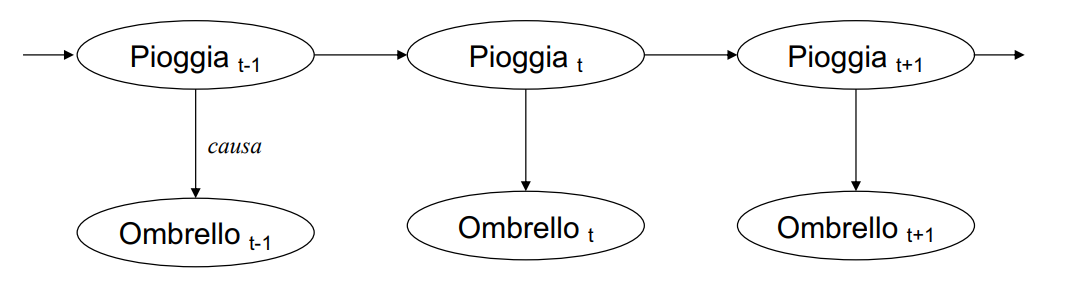
\includegraphics[width=.5\textwidth]{img/catene/hmm.png}
    \caption{Esempio di catena di Markov a stati nascosti}
    \label{fig:HMM}
\end{figure}

Secondo questo grafico potrebbero esserci problemi legati alla presenza di infinite 
CPT, in realtà no perché si ha l'assunzione di \textbf{stazionarietà} (i cambiamenti 
sono regolati da leggi immutabili nel tempo). In aggiunta si potrebbe pensare di 
che ci siano infiniti genitori per ogni stato, in realtà no perché si ha l'assunzione 
di \textbf{ipotesi di Markov} (lo stato corrente dipende solo da una storia finita 
degli stati precedenti).

Si potrebbe pensare che l'\textbf{ipotesi di Markov} sia troppo stringente, per 
rimediare possiamo aumentare l'ordine del modello di processo di Markov oppure di 
aumentare l'insieme delle variabili di stato.

\subsection{Inferenza}
L'inferenza con questi modelli è di $4$ tipologie:
\begin{itemize}
    \item \textbf{filtraggio}: calcolo $X_t$ dato tutte le osservazioni del passato $e_{1:t}$
    $$P(X_t | e_{1:t})= f(e_t, P(X_{t-1}|e_{1:t-1}))$$
    Le osservazioni si fanno partire da $1$ perché si può scegliere se raccoglierle 
    da $1$ a $0$.
    In sostanza si parte $t=0$ si effettua la predizione dello stato a $t+1$ dato 
    lo stato $t$ (proiezione), poi aggiorno la probabilità allo stato $t+1$ con 
    l'osservazione $t+1$ data (aggiornamento). Si rieseguono i passi ricorsivamente
    fino al tempo scelto.

    Generalizzando a $t' \in \{0,t-1\}$, per calcolare un generico $P(X_{t'+1}|e_{1:t'+1})$
    dobbiamo: 
    $$P(X_{t'+1} | e_{1:t'+1}) = P(X_{t'+1} | e_{1:t'}, e_{t'+1})= \alpha P(e_{t'+1}|X_{t'+1}, e_{1:t'})\cdot P(X_{t'+1}|e_{1:t'})=$$
    $$=\alpha P(e_{t'+1}|X_{t'+1})\cdot P(X_{t'+1}|e_{1:t'}) $$
    La formula si ottiene prima separando l'evidenza al termpo $t'+1$ rispetto al tempo $t'$,
    successivamente è stata utilizzata la regola di Bayes e successivamente l'assunzione 
    di indipendenza tra $e_t'$ e $e_{t'+1}$ ($\alpha$ costante di normalizzazione). 
    
    Quindi
    $$P(X_{t'+1} | e_{1:t'+1}) =\alpha P(e_{t'+1}|X_{t'+1})\cdot P(X_{t'+1}|e_{1:t'}) = 
    =\alpha P(e_{t'+1}|X_{t'+1})\cdot \sum_{x_{t'}}P(X_{t'+1}|x_{t'},e_{1:t'}) P(x_{t'}|e_{1:t'})$$
    Dove $x_{t'}$ sono gli stati possibili al tempo $t'$.

    
    \item \textbf{previsione}: coincide col filtraggio privo dell'aggiunta di nuove 
    osservazioni. Coincide col calcolare 
    $$P(X_{t+k } | e_{1:t})$$ 

    Quando tentiamo di predire ad istanti di tempo molto più avanti, maggiore 
    sarà l'incertezza del modello di transizione, più breve sarà il tempo per raggiungere
    un punto fisso per una predizione (distribuzione stazionaria) e più ignoto sarà il futuro.
    \item \textbf{smoothing}: correggo gli stati passati avendo osservato le variabili 
    fino oggi. Aggiorniamo gli stati del passato con le osservazioni del passato e del 
    futuro. 
    $$P(X_k | e_{1:t}), \forall 1\le k < t$$

    Il calcolo coincide con
    $$P(X_k | e_{1:t}) = P(X_k | e_{1:k}, e_{k+1:t}) = \alpha P(X_{k}|e_{1:k}) P (e_{k+1:t}|X_k,e_{1:k}) = \alpha P(X_{k}|e_{1:k}) P (e_{k+1:t}|X_k)$$
    Si sfrutta la regola di Bayes e l'indipendenza condizionata.

    $$P(X_k | e_{1:t}) =\alpha P(X_{k}|e_{1:k}) P (e_{k+1:t}|X_k) =\alpha f_{1:k}b_{k+1:t} $$
    Dove $f_{1:k}$ consiste nel filtrare in avanti da $1:k$ mentre $b_{k+1:t}$ viene 
    calcolato mediante la procedura ricorsiva di backward che procede all'interno di $t$.

    $$b_{k+1:t} = P(e_{k+1:t}|X_k)=\sum_{x_{k+1}} P (e_{k+1:t}|X_k,x_{k+1}) P (x_{k+1}|X_k)=\sum_{x_{k+1}} P (e_{k+1:t}|x_{k+1}) P (x_{k+1}|X_k)=$$
    $$\sum_{x_{k+1}} P (e_{k+1},e_{k+2:t}|x_{k+1}) P (x_{k+1}|X_k) =\sum_{x_{k+1}} P (e_{k+1}|x_{k+1}) P(e_{k+2:t} | x_{k+1}) P (x_{k+1}|X_k)$$
    
    Complessità spaziale molto elevata perché si hanno molti stati e sequenze lunghe e 
    incapacità di lavorare in ambienti online (si risolve con smoothing a ritardo fisso).
    \item \textbf{spiegazione più probabile}: data una sequenza di osservazioni
    vogliamo trovare la sequenza di stati che più probabilmente ha generato il mio
    set di osservazioni.
    $$\arg\max_{x_1:t} P(x_{1:t}|e_{1:t})$$
    Supponiamo di essere in stati binari e che la sequenza delle osservazioni sono $n$,
    questo significa che abbiamo $2^n$ possibili sequenze di stati. Utilizzeremo 
    l'algoritmo di \textbf{Viterbi} che si basa sull'assunzione che esiste una 
    relazione ricorsiva fra i cammini più probabili verso lo stato $x_{t+1}$ e i 
    cammini più probabili verso ogni stato $x_t$. Ovvero significa dire
    $$\max _{x_1,\dots, x_t} P(x_1,\dots,x_t,X_{t+1}|e_{1:t+1})= \alpha P(e_{t+1})\max_{x_t} \{P(X_{t+1}|x_t)\max_{x_1,\dots,x_{t-1}} \{P(x_1,\dots,x_{t-1},x_t|e_{1:t})\}\}$$
\end{itemize}
